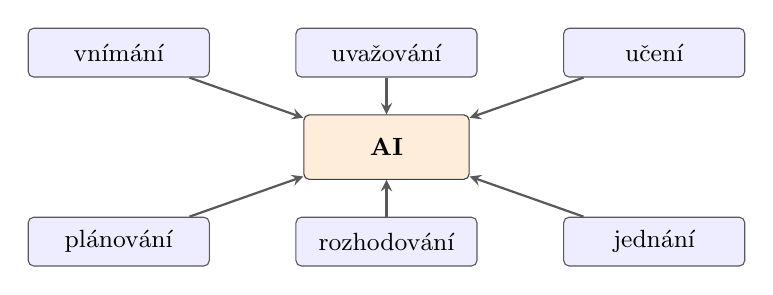
\begin{tikzpicture}[
    >=stealth,
    concept/.style={
        draw=black!65,
        rounded corners=2pt,
        fill=blue!7,
        minimum width=2.3cm,
        minimum height=0.62cm,
        align=center,
        font=\small
    },
    ai/.style={
        draw=black!75,
        rounded corners=2pt,
        fill=orange!14,
        minimum width=2.1cm,
        minimum height=0.82cm,
        align=center,
        font=\small\bfseries
    },
    arr/.style={->, thick, draw=black!65}
]
    \node[concept] (perception) at (-3.4,1.2) {vnímání};
    \node[concept] (reasoning) at (0,1.2) {uvažování};
    \node[concept] (learning) at (3.4,1.2) {učení};

    \node[ai] (ai) at (0,0) {AI};

    \node[concept] (planning) at (-3.4,-1.2) {plánování};
    \node[concept] (decision) at (0,-1.2) {rozhodování};
    \node[concept] (acting) at (3.4,-1.2) {jednání};

    \draw[arr] (perception) -- (ai);
    \draw[arr] (reasoning) -- (ai);
    \draw[arr] (learning) -- (ai);
    \draw[arr] (planning) -- (ai);
    \draw[arr] (decision) -- (ai);
    \draw[arr] (acting) -- (ai);
\end{tikzpicture}
